\documentclass[conference]{IEEEtran}

\usepackage[utf8]{inputenc}
\usepackage{cite}
\usepackage{graphicx}
\graphicspath{{figs/}}
\DeclareGraphicsExtensions{.pdf,.jpg,.png}

\usepackage[caption=false,font=footnotesize]{subfig}
\usepackage{url}
\hyphenation{op-tical net-works semi-conduc-tor}


\begin{document}
%
% paper title
% can use linebreaks \\ within to get better formatting as desired
\title{Natural Interaction for Object Hand-Over}


\author{\IEEEauthorblockN{Mamoun Gharbi, Séverin Lemaignan, Jim Mainprice, Rachid Alami}
\IEEEauthorblockA{CNRS-LAAS, 7 av. du Colonel Roche, F-31077 Toulouse, France\\
Université de Toulouse, UPS, INSA, INP, ISAE, LAAS, F-31077 Toulouse, France\\
Email: {\tt surname.name@laas.fr}}
}
% make the title area
\maketitle


\begin{abstract}

The video presents in a didactic way several of the abilities and algorithms
required to achieve interactive "pick and place" tasks in a human environment.
Communication between the human and the robot relies on unconstrained verbal
dialogue, the robot relies on multi-modal perception to track the human and its
environment, and implements real-time 3D motion planning algorithms to achieve
collision-free and human-aware interactive manipulation.

\end{abstract}


\section{The challenges of natural interactive manipulation}

%This film covers recent results from the LAAS-CNRS laboratory in the field of
%\emph{interactive manipulation with companion robots}. 
Our challenge exhibited here is \emph{natural} and \emph{legible} behaviour for a robot intended to 
live in human environment, amongst human peers.
\emph{Natural} because we aim at unconstrained spoken English mixed with
gestures and perspective taking to communicate with the robot ; \emph{legible}
because we apply human-aware motion planning algorithms that ensure a smooth human-robot interaction by accounting for implicit social rules which appear in placement or approach strategies.

\section{Main demonstrated abilities and algorithms}

The video demonstration is the result of the integration of many different
components. Besides {\it off the shelf} PR2 components (like the laser-based
localisation or the 2D navigation), we introduce here (Fig.~\ref{fig|archi})
several new components focuses on higher level planning and decision making.

\begin{figure}[h!]
        \centering
        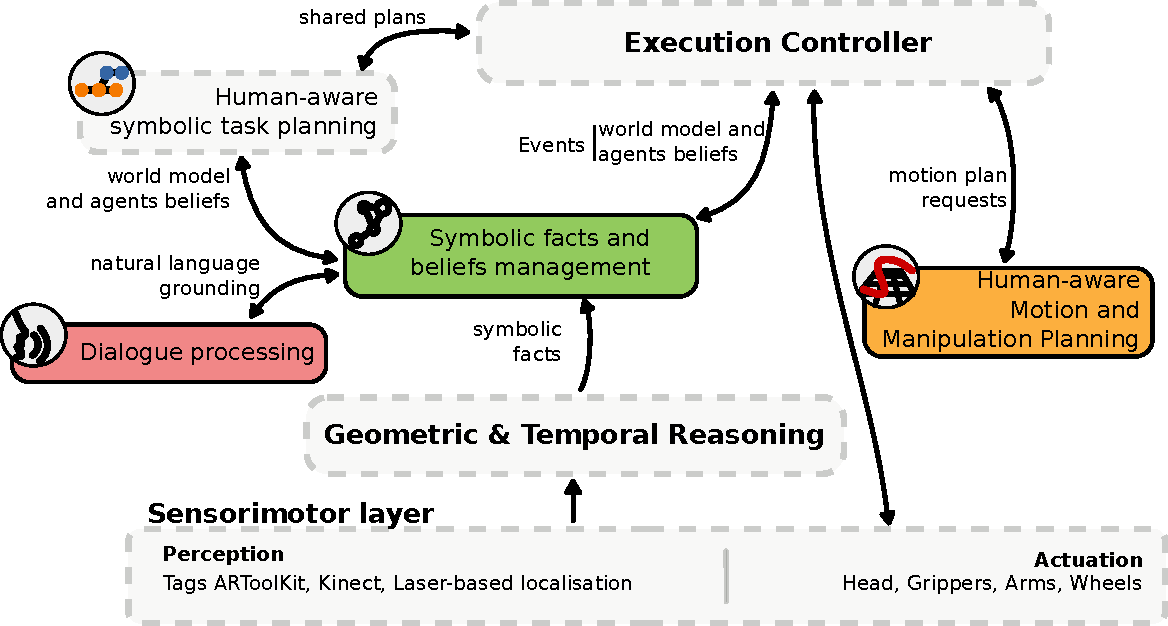
\includegraphics[width=\columnwidth]{archi}
        \caption{Overview of the robot deliberative
        architecture~\cite{Alami2011a}. Coloured modules with plain borders are
        a specific focus of the video.}
        \label{fig|archi}
\end{figure}

\subsection{Modelling of the environment}

The film gives a overview of some of the techniques used on-line by the robot
to build a model of its environment. We rely first on a geometric model, fed by
Kinect-like sensors for human tracking, 2D barcodes for object identification
and localization, and the PR2 own laser-based localization.

From this geometric model, we build in real-time a symbolic model, stored as an
ontology~\cite{Lemaignan2010}. This models holds spatial relations between
objects and agents, along with a set of \emph{affordances} (like reachability,
visibility, etc.). The system is able to store independent symbolic models for
each agents through \emph{perspective taking} techniques.

\subsection{Natural language processing}

The video also introduces recent work on natural dialogue
grounding~\cite{Lemaignan2011a}. The user verbal input is converted to text via
a custom Android application, and send to the robot where we first parse, then
semantically ground the user input, in tight interaction with the symbolic
model. This allows for instance multi-modal communication: human gestures that
are recognized (like pointing) and stored in the ontology can be used during
the grounding process.

\subsection{Human-aware motion planning for hand-over}

The handover planning problem as formalized in \cite{Mainprice:12} demonstrates the necessity to account for the human motion in the planning process. Indeed in situation where the human is not directly accessible to the robot, it is important to ensure that the human is able to reach the handover location. Then the problem resides in where the handover should take place given that some positions might lead to more human effort or be more time consuming and thus less fluent. We have introduced a parameter we call \textit{mobility} of the human receiver to balance between comfort and efficiency of the handover. The proposed planner combines grid-based and sampling-based approaches into an efficient solution.
%\subsection{Human-aware trajectory planning for hand-over}

\subsection{Manipulation planning in close human vicinity}

Object handovers require manipulation from the robot part. To achieve this task safely and in a human friendly manner it is important to account for interaction constraints such as defined by the "proxemixs" theory. The motion planning techniques we have introduced in \cite{Mainprice:11}  enable to account for such constraints by incorporating features from stochastic optimization to cope with the complexity of the cost-based motion planning problem. They enable to produce safe plans for full body approach motions or manipulation in highly cluttered scenes.

\section*{Acknowledgment}

This work has been partially funded by EU project SAPHARI.

\bibliographystyle{IEEEtran}
\bibliography{IEEEabrv,biblio,bib_jim}

% that's all folks
\end{document}


